\documentclass[border=10pt]{standalone}

\usepackage{tikz}
\usepackage{tikzsymbols}
\usetikzlibrary{calc,patterns,shapes.geometric}

\def\centerarc[#1](#2)(#3:#4:#5){\draw[#1] ($(#2)+({#5*cos(#3)},{#5*sin(#3)})$) arc (#3:#4:#5);}

\begin{document}
	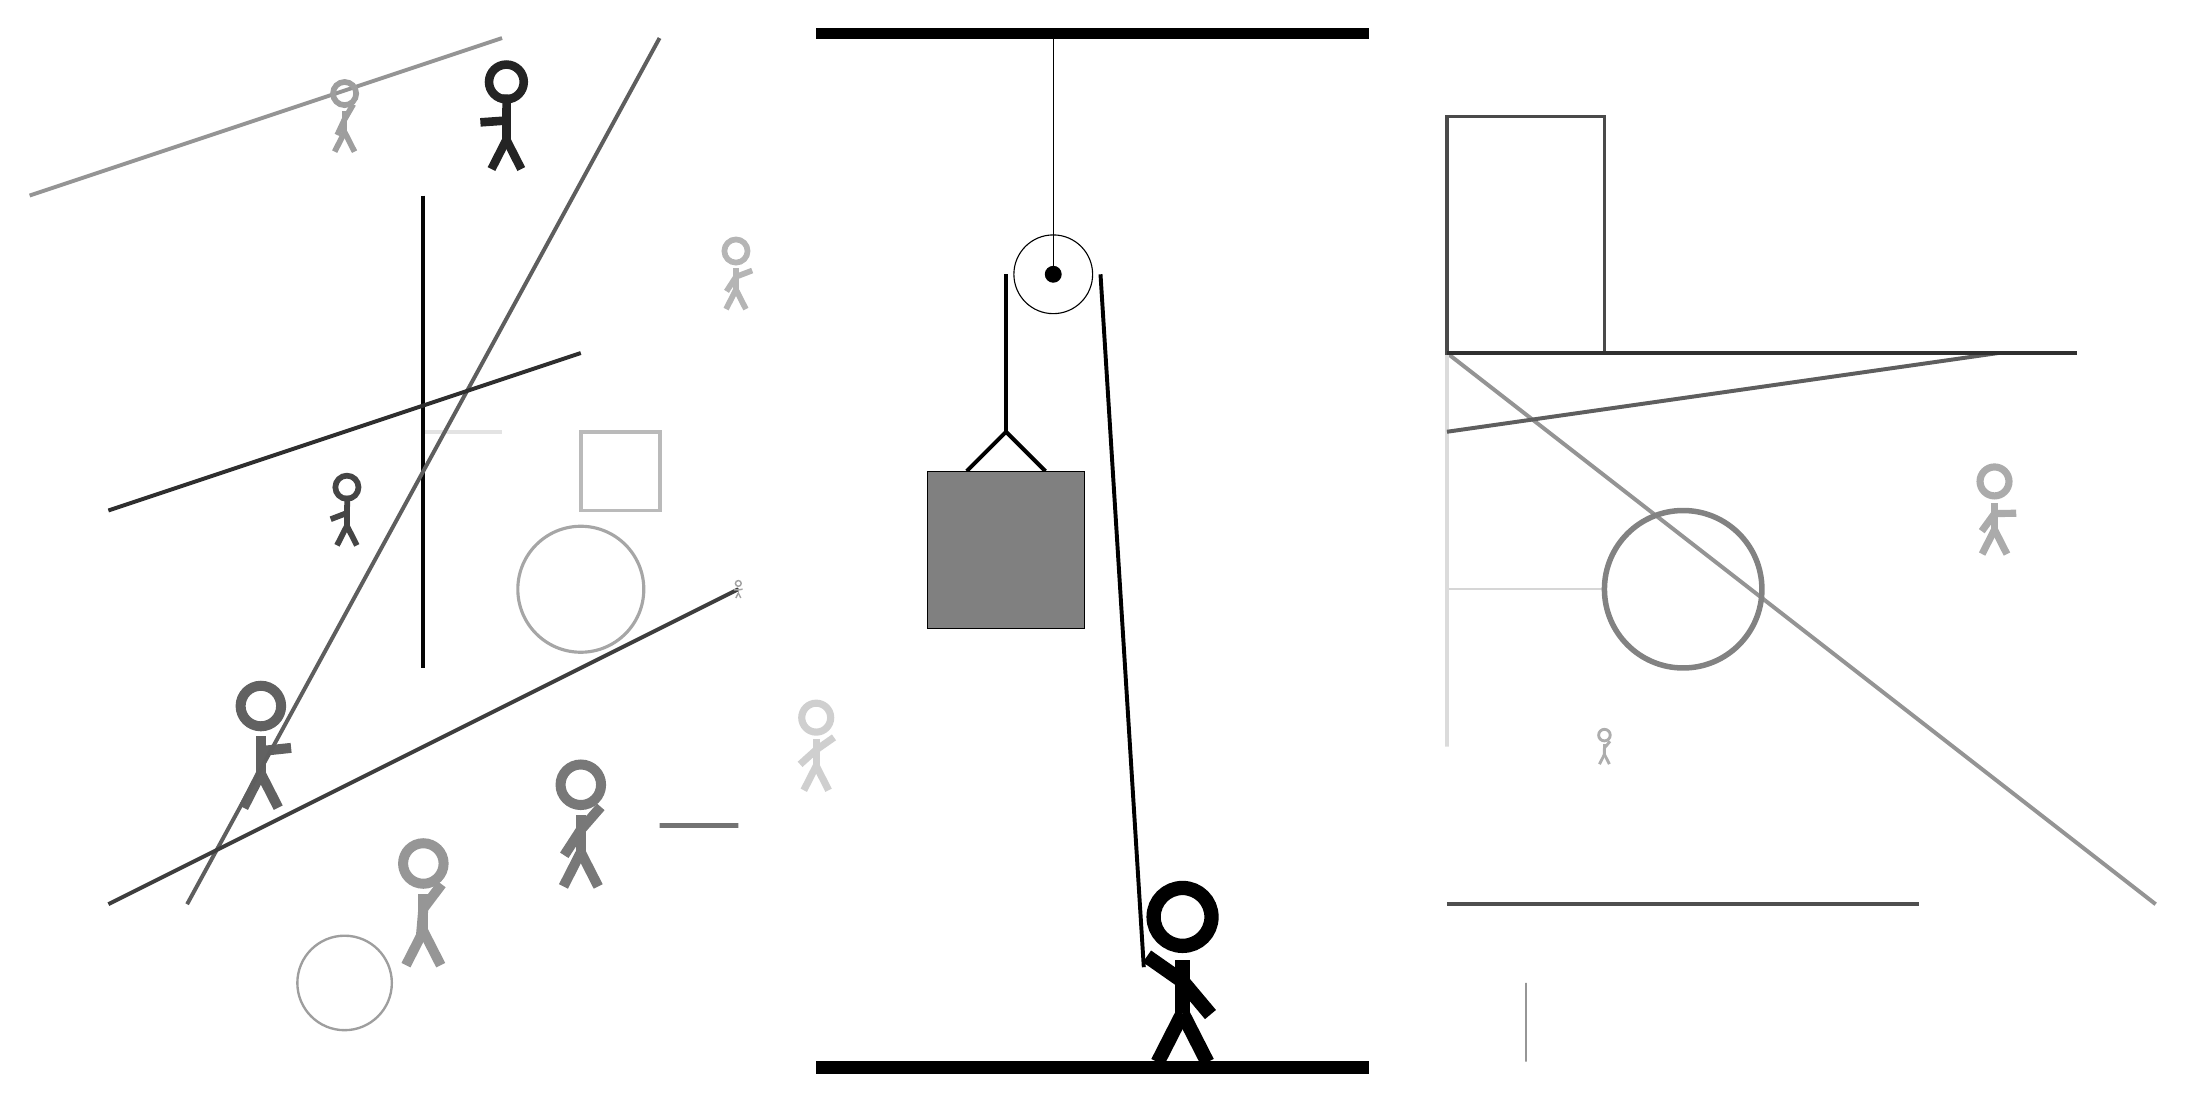
\begin{tikzpicture}
		%%%%% START %%%%%
		
		\draw[fill=black] (-2, 10) rectangle (5, 10.125);
		
		\draw (1, 7) circle (0.5);
		\draw[fill=black] (1, 7) circle (0.1);
		\draw (1, 10) -- (1, 7);
		
		\draw[line width=0.5mm] (-0.1, 4.5) -- (0.4, 5.0) -- (0.9, 4.5);
		\draw[fill=black!50] (-0.6, 4.5) rectangle (1.4, 2.5);
		
		\draw[line width=0.5mm] (0.4, 7) -- (0.4, 5.0);
		\centerarc[line width=0.5mm](1, 7)(0:180:0.6);
		\draw[line width=0.5mm](1.6, 7) -- (2.15, -1.8);
		
		\node[line width=0.7mm, color=black!33] at (13, 4) {\Strichmaxerl[5][54][1]};
		
		\node[line width=0.4mm, color=black!62] at (-9, 1) {\Strichmaxerl[7][90][6]};
		\node[line width=0.3mm, color=black!73] at (-8, 4) {\Strichmaxerl[4][21][88]};
		\draw[line width=0.5mm, color=black!11](-7, 5) -- (-6, 5);
		
		\draw[line width=0.5mm, color=black!42](-6, 10) -- (-12, 8);
		\draw [line width=0.3mm, color=black!38](-8, -2) circle (0.6);
		\draw[line width=0.5mm, color=black!98](-7, 8) -- (-7, 2);
		
		\draw[line width=0.2mm, color=black!16] (6, 3) rectangle (8, 3);
		\node[line width=0.2mm, color=black!53] at (-5, 0) {\Strichmaxerl[7][57][49]};
		\node[line width=0.4mm, color=black!29] at (-3, 7) {\Strichmaxerl[4][57][21]};
		\draw[line width=0.5mm, color=black!42](6, 6) -- (15, -1);
		\node[line width=0.6mm, color=black!32] at (8, 1) {\Strichmaxerl[2][88][50]};
		\draw[line width=0.6mm, color=black!14] (6, 9) rectangle (6, 1);
		\draw[line width=0.5mm, color=black!27] (-4, 4) rectangle (-5, 5);
		\draw[line width=0.6mm, color=black!55] (-4, 0) rectangle (-3, 0);
		\draw[line width=0.4mm, color=black!71] (6, 6) rectangle (8, 9);
		
		\draw[line width=0.5mm, color=black!63](-4, 10) -- (-10, -1);
		\node[line width=0.7mm, color=black!41] at (-7, -1) {\Strichmaxerl[7][85][53]};
		\draw [line width=0.4mm, color=black!35](-5, 3) circle (0.8);
		
		\draw[line width=0.5mm, color=black!63](6, 5) -- (13, 6);
		\draw[line width=0.3mm, color=black!41] (7, -3) rectangle (7, -2);
		
		\draw[line width=0.5mm, color=black!69](6, -1) -- (12, -1);
		
		\draw[line width=0.5mm, color=black!82](-5, 6) -- (-11, 4);
		\node[line width=0.4mm, color=black!19] at (-2, 1) {\Strichmaxerl[5][42][35]};
		\draw[line width=0.5mm, color=black!76](-3, 3) -- (-11, -1);
		
		\draw [line width=0.7mm, color=black!49](9, 3) circle (1.0);
		\node[line width=0.2mm, color=black!37] at (-3, 3) {\Strichmaxerl[1][1][9]};
		\draw[line width=0.5mm, color=black!81](6, 6) -- (14, 6);
		\node[line width=0.6mm, color=black!86] at (-6, 9) {\Strichmaxerl[6][4][89]};
		\node[line width=0.3mm, color=black!38] at (-8, 9) {\Strichmaxerl[4][65][60]};
		
		\node at (2.6, -1.9) {\Strichmaxerl[10][-35][-50]};
		
		\draw[fill=black] (-2, -3) rectangle (5, -3.15);
		
		%%%%% END %%%%%
	\end{tikzpicture}
\end{document}